% 图 8.7 一维海森伯反铁磁链自旋子（spinon）连续谱：
% 下边界 hbar*omega = pi*J|sin(qa)|（粗线），上边界 2*pi*J|sin(qa)|（细线），之间斑点状连续谱
\documentclass[tikz,border=5pt]{standalone}
\usetikzlibrary{arrows.meta,patterns}
\usepackage{amsmath}
\usepackage{bm}
\usepackage{fontspec}
\setmainfont{Times New Roman}
% speckle pattern for the continuum
\pgfdeclarepatternformonly{speckle}{\pgfpointorigin}{\pgfpoint{5pt}{5pt}}{\pgfpoint{5pt}{5pt}}{
  \pgfsetcolor{black!72}
  \pgfpathcircle{\pgfpoint{0.8pt}{1.2pt}}{0.55pt}
  \pgfpathcircle{\pgfpoint{2.7pt}{3.5pt}}{0.6pt}
  \pgfpathcircle{\pgfpoint{4.2pt}{0.7pt}}{0.5pt}
  \pgfpathcircle{\pgfpoint{1.7pt}{4.4pt}}{0.45pt}
  \pgfpathcircle{\pgfpoint{3.9pt}{2.3pt}}{0.4pt}
  \pgfusepath{fill}}
\begin{document}
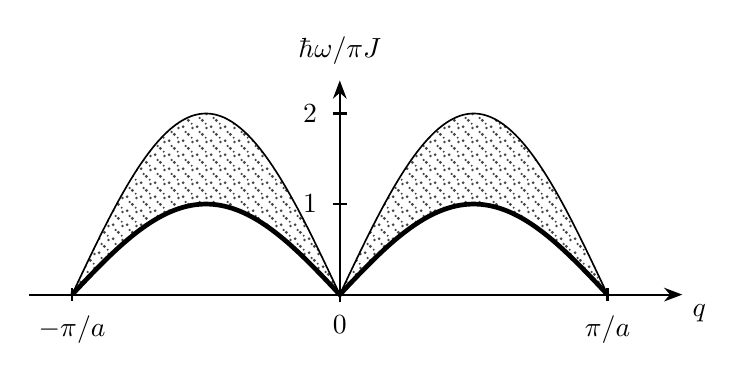
\begin{tikzpicture}[line width=0.8pt,>=Stealth]
  % shaded continuum between the two boundaries
  \fill[pattern=speckle]
    plot[domain=-180:180,samples=181,smooth]
      ({3.4*\x/180},{1.15*abs(sin(\x))})
    -- plot[domain=180:-180,samples=181,smooth]
      ({3.4*\x/180},{2.30*abs(sin(\x))})
    -- cycle;
  % boundaries: lower bold, upper thin
  \draw[line width=1.7,domain=-180:180,samples=181,smooth]
    plot ({3.4*\x/180},{1.15*abs(sin(\x))});
  \draw[line width=0.6,domain=-180:180,samples=181,smooth]
    plot ({3.4*\x/180},{2.30*abs(sin(\x))});
  % axes
  \draw[->] (-3.95,0) -- (4.35,0) node[below right]{$q$};
  \draw[->] (0,-0.10) -- (0,2.72);
  \node[above=2pt] at (0,2.72) {$\hbar\omega/\pi J$};
  % y ticks 1 and 2
  \draw[line width=0.9] (-0.09,1.15) -- (0.09,1.15);
  \node[left] at (-0.16,1.15) {$1$};
  \draw[line width=0.9] (-0.09,2.30) -- (0.09,2.30);
  \node[left] at (-0.16,2.30) {$2$};
  % x labels
  \draw[line width=0.9] (-3.4,-0.08) -- (-3.4,0.08);
  \node[below] at (-3.4,-0.14) {$-\pi/a$};
  \node[below] at (0,-0.14) {$0$};
  \draw[line width=0.9] (3.4,-0.08) -- (3.4,0.08);
  \node[below] at (3.4,-0.14) {$\pi/a$};
\end{tikzpicture}
\end{document}
